\section{Methodology}\label{sec:meth}
Mathematical models of the type considered above in Section~\ref{sec:intro} contain both {\sl state variables} $\mathbf y = (y_1, \dots, y_N)$  and {\sl uncertain parameters} $\boldsymbol{\theta} = (\theta_1, \dots, \theta_P)$. The evolution of the state variables is governed by a system of ordinary differential equations (ODEs) 
\begin{eqnarray}
\frac {d\boldsymbol{y}}{dt} = \mathbf{f}(\mathbf{y}, \boldsymbol{\theta}), \label{caboodle}
\end{eqnarray}
where $\mathbf{f}$ is a known function of its arguments. For our model, there are $N = 67$ state variables and $P=160$  parameters that we regard as uncertain. 

\todo[inline]{SAY SOMETHING ABOUT ICS}

As is the case for most applications, the mathematical model is considered as a way to evaluate and analyze {\sl Quantities of Interest} (QoIs) whose behavior is key to the qualitative and/or quantitative understanding of the phenomenon of under consideration; any such QoI $q$ is determined from the state variables and is thus, ultimately, a function of the parameters alone (and possibly time), i.e.
\begin{eqnarray}
q = g(\boldsymbol{\theta}). \label{qoi}
\end{eqnarray}
The overall goal of our numerical study is to determine  which of the uncertain parameters $\theta_1, \dots, \theta_{160}$  are the most/least influential on a chosen QoIs $q$ of the type (\ref{qoi}). 



\subsection{Numerical experimental setup}
The numerical experiments solve (\ref{caboodle}) in the presence of short duration electrical stimuli as displayed in Figure~\ref{input_stimuli}.

\todo[inline]{EXPLAIN THIS BETTER, LINK TO SPECIFIC STATE VARIABLE AND MODEL}

\begin{figure}[h]
\centering
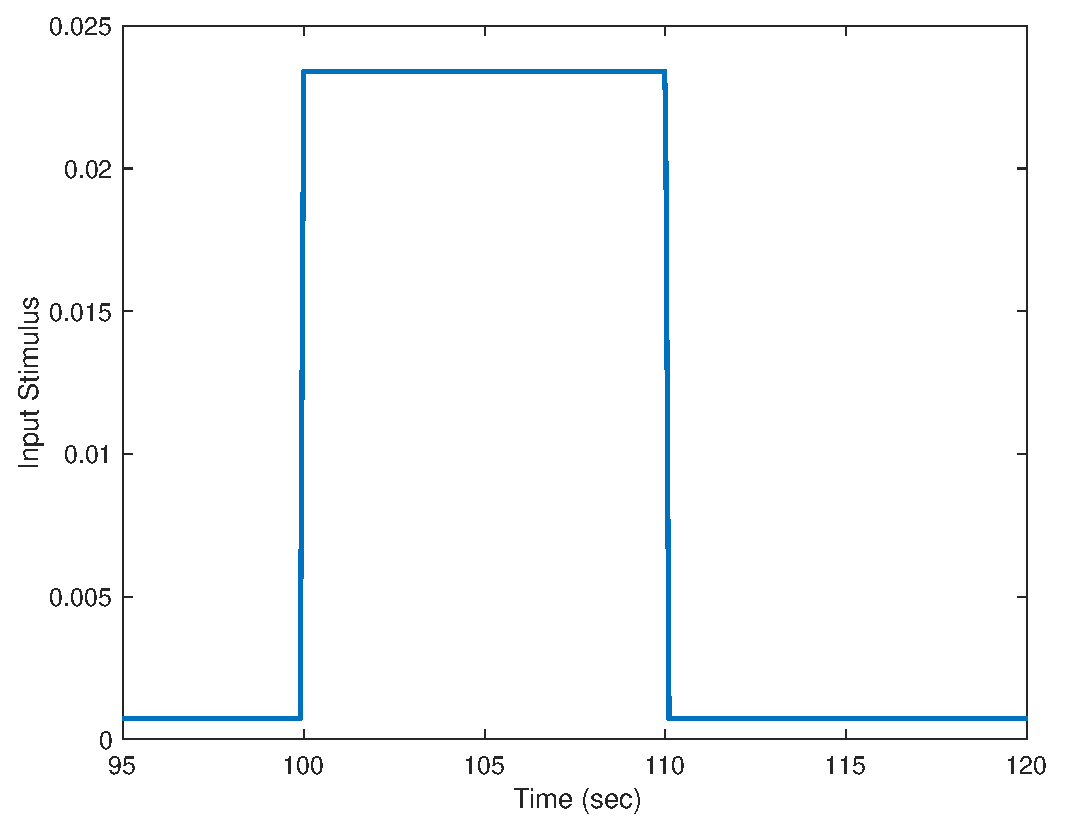
\includegraphics[width=.4 \textwidth]{Figures/Rectangular_Stimulus.eps}
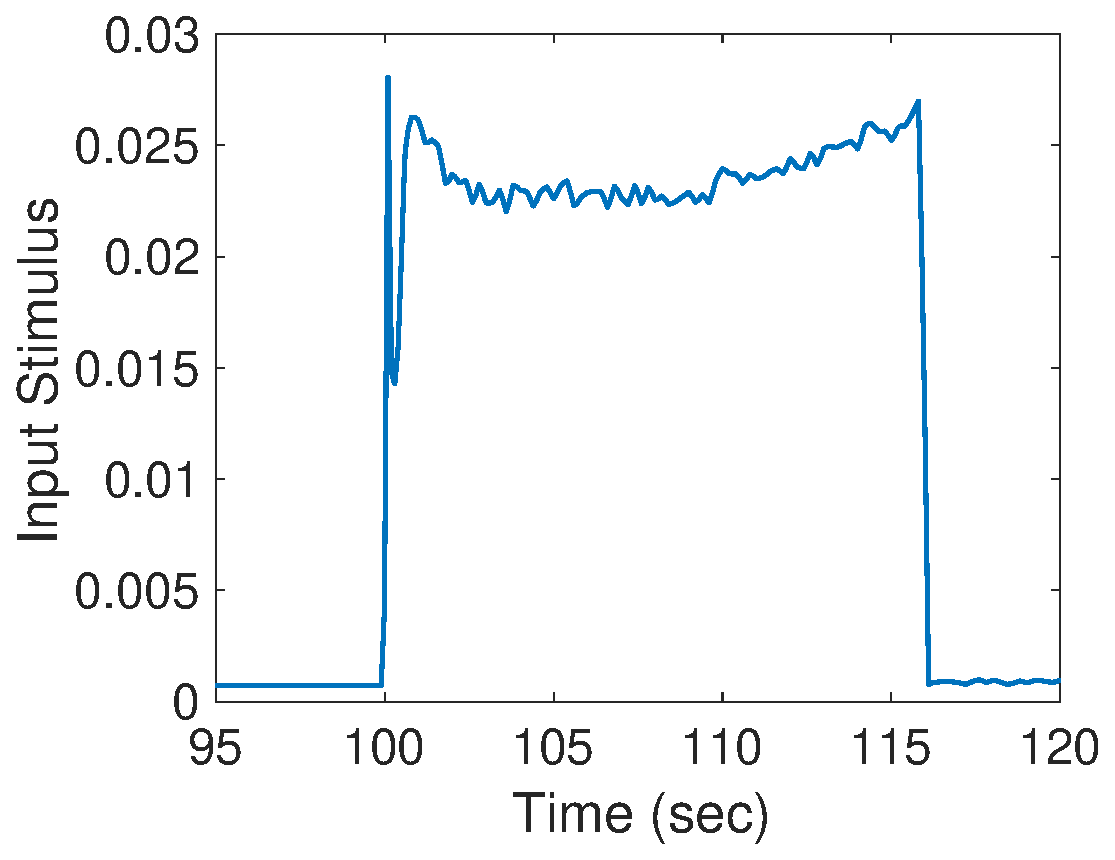
\includegraphics[width=.4 \textwidth]{Figures/Experimental_Stimulus.eps}
\caption{Left: rectangular pulse input stimulus; right: stimulus used in lab experiments.}
\label{input_stimuli}
\end{figure}

 Assuming the stimulation occurs for $t_1\le t \le t_2$, the QoIs are defined as follows
 \begin{itemize}
\item average ECS potassium 
\begin{eqnarray}
%[K^+]_{max,ECS} \label{K_ECS_Max} \\
 q_1 = \frac{1}{t_2-t_1}\int_{t_1}^{t_2}[K^+]_{ECS}(s)\, ds, \label{K_ECS_Mean}
\end{eqnarray}
\item average volumetric flow rate in the cerebral tissue
\begin{equation}
 q_2 = \frac{1}{t_2-t_1}\int_{t_1}^{t_2}\left(\frac{R(s)}{R_0}\right)^4\, ds, \label{vol_flow}
\end{equation}
 \item minimum combined concentration of the actin myosin complex, both phosphorylated and unphosphorylated
\begin{eqnarray}
q_3 = \min _{t, t_1\le t \le t_2} [AM+AM_p]. \label{AM_AMp_Min}
\end{eqnarray}
\end{itemize}

An important decision (and delicate) {\sl modeling} decision  is how to describe the uncertainty attached to the parameter vector $\boldsymbol{\theta}$. Here, we give each $\theta_i$, $i=1,\dots, 160$, a nominal value $\bar \theta_i$ and assume each parameter to be uniformly distributed over the range of value $[0.9\, \bar\theta_i, 1.1 \,\bar\theta_i]$, i.e., within $\pm 10\%$ of the nominal value. All the parameters for now are assumed to be independent, an assumption we revisit and improve upon below. 

\todo[inline]{SOME OF THE DISCUSSION OF THE "RESULT SECTION" ABOUT SAMPLING SHOULD BE MOVED HERE}

A key  step in analyzing the dependency of a QoI $q = g(\boldsymbol{\theta})$ on its inputs is the evaluation of $g$ at $M$ samples $\boldsymbol\theta^k$, $k=1,\dots, M$, from the parameter distribution (where superscripts are used to refer to specific samples). 
This is also the  main  computational bottleneck as it requires the numerical resolution of  the ODE system (\ref{caboodle})  by computing the $M$ solutions $\mathbf y^k$, $k=1,\dots , M$, corresponding to  the parameter samples. 
While relatively large and stiff, the ODE system (\ref{caboodle}) can be  solved with standard tools and methods, here through the MATLAB routine ode15s  with relative and absolute tolerances of $10^{-4}$. The evaluation of the above QoIs themselves from the ODE solutions is straightforward and can be done at low cost.

There is substantial amount of research currently being done in applied mathematics and statistics on GSA. How to meaningfully define ``influential" or ``non-influential" and  how to develop methods applicable to high-dimensional problems are two significant challenges of the field. 

\todo[inline]{CITE SOMETHING}


For the present application, the large parameter dimension and computational cost of the above model evaluations prohibit the direct use of most global sensitivity analysis methods. In other words, the value of $M$ (number of samples)  we can ``afford" is too small for these methods to be applicable. 
For each QoI, the overall procedure is thus as follows. 

\begin{enumerate}
\item[(i)] dimension reduction,
\item[(ii)] surrogate modeling,
\item[(iii)] global sensitivity analysis.
\end{enumerate}

These steps are individually considered in the next three subsections. 




\subsection{Dimension reduction}
Using the previously generated model evaluations, we fit a {\sl linear model} to a QoI under study
\begin{eqnarray}
g(\boldsymbol\theta^k) = g(\theta_1^k, \dots, \theta_P^k) \approx \beta_0 + \sum\limits_{j=1}^{160} \beta_j \theta_j^k, \quad j=1, \dots, M. \label{lr}
\end{eqnarray}
This approach yields a crude (but highly efficient here) sensitivity analysis of the model with respect to the $\theta_j$'s, $j=1,\dots, 160$. We assign a preliminary importance measure to each $\theta_j$ by computing for each of them the relative size of their coefficient in the above linear approximation, i.e.
\begin{eqnarray*}
L_j = \frac{\vert \beta_j \vert}{\sum\limits_{\ell=1}^{160} \vert \beta_\ell \vert}, \qquad k=1,\dots,160.
\end{eqnarray*}
To obtain a model with a more manageable size, we reduce the parameter space to only the $\theta_j$'s for which $L_j>0.01$. We denote these $r$ parameters $\{ \theta_{j_i}\}_{i=1}^r$. The rest of the parameters are regarded as non-influential and set to their nominal values since, even though they are uncertain, their specific values (within the given range) have little bearing of the considered QoI. In other words, we consider the approximation 
\begin{eqnarray}
g(\theta_1, \dots, \theta_{160}) \approx h(\theta_{j_1}, \dots, \theta_{j_r}), \label{reddim}
\end{eqnarray}
where $h$ is obtained from $g$ by fixing any non-influential parameter $\theta_j$ in $g$  to its nominal value $\bar\theta_j$. In Section~\ref{sec:results}, this reduction yields around $15-20$ parameters instead of the original 160. 


\subsection{Surrogate model}
For any of the three considered QoIs, our information on the function $h$ defined (\ref{reddim}) consists of the set of sampled values $\{ h(\theta_{j_1}^k, \dots, \theta_{j_r}^k)\}$, $k=1, \dots, M$.  To facilitate the use of standard GSA tools, which may require derivatives or variance estimations, it is both convenient and computationally advantageous to construct an approximating function, i.e., a surrogate model. 
We use a sparse Polynomial Chaos (PC) surrogate. This amounts to introducing a polynomial approximation of $h$ of the type
\begin{eqnarray}
h(\boldsymbol{\theta}) \approx \sum_{\boldsymbol{\alpha}} c_{\boldsymbol{\alpha}} \psi_{\boldsymbol{\alpha}}(\boldsymbol{\theta}) \label{pce}
\end{eqnarray}
where the $\psi_{\boldsymbol{\alpha}}$'s are multivariate polynomials which are orthogonal with respect to the probability distribution function (PDF) $p_{\boldsymbol{\theta}}$ of $\boldsymbol{\theta}$, i.e.
\begin{eqnarray}
\int \psi_{\boldsymbol{\alpha}}(\mathbf x) \psi_{\boldsymbol{\beta}}(\mathbf x)\, p_{\boldsymbol{\theta}}(\mathbf x) \, d\mathbf{x} = \delta _{\boldsymbol{\alpha},\boldsymbol{\beta}} \label{ortho}
\end{eqnarray}
where $\boldsymbol{\alpha}$ and $\boldsymbol{\beta}$ are multi-indices and $\delta _{\boldsymbol{\alpha}}$ is the generalized Kronecker symbol. Due to our choice of distributions for $\boldsymbol{\theta}$, the $\psi_{\boldsymbol{\alpha}}$'s are essentially Legendre polynomials and the coefficients are computed through least-squares minimization. All surrogate models are validated using 10-fold cross validation.

Polynomial chaos is by now a well documented method and we refer the readers for instance to the  UQLab \cite{uqlab} manual for more details. Incidentally, we make use of the implementation from  \cite{uqlab} in the results below. 


\subsection{Global sensitivity analysis} 

\todo[inline]{still to do....}

The total Sobol' indices \cite{saltellitotalindex} of the PC surrogate are computed to yield a quantitative measure of importance for each $\theta_{k_i}$, $i=1,2,\dots,r$.


